\section{Lecture 4: Understanding the Impostor Terms}

\subsection{Introduction}
We have talked about how sampling a signal can create impostor terms. As discussed previously, these impostor terms have the same values at the sampled points, but are in essence different signals all together. We also looked at the impostor terms for when the original signal is a sinusoid and the impostor terms are also sinusoids. In this lecture, we will carry this discussion forward and see how the different sinusoids act all together.

\subsection{Adding the sinusoid terms}
\noindent Recall that the sinusoid terms can be written as follows:-
\[
A_{0} \cos \left (2\pi(\frac{k}{T_{s}}-\frac{1}{T_{0}})t - \frac{\pi}{4}\right)
\]
\[
A_{0} \cos \left (2\pi(\frac{k}{T_{s}}+\frac{1}{T_{0}})t + \frac{\pi}{4}\right)
\]

\noindent where k is any positive integer.

\noindent A sum of the original signal and all the impostor terms will look like:-

\[
A_{0} \cos \left (2\frac{\pi}{T_{0}}t+\frac{\pi}{4}\right) + \sum_{k=1}^{N}\left( A_{0} \cos \left (2\pi(\frac{k}{T_{s}}-\frac{1}{T_{0}})t - \frac{\pi}{4}\right)+ A_{0} \cos \left (2\pi(\frac{k}{T_{s}}+\frac{1}{T_{0}})t + \frac{\pi}{4}\right)\right)
\]
where N \textgreater 0
\\
At this point, the following substitution will make it easier to work out the math.
\[
B=\frac{2\pi k}{T_{s}}
\ and
\
C=\frac{1}{T_{0}} + \frac{\pi}{4}
\]
 Notice that the term C is independent of k.
 For a given k, the sum inside the $\Sigma$ reduces to 
\[ A_{0}\cos (B-C) + A_{0}\cos (B+C) = 2A_{0}\cos B\cos C
\]
This will make the sum :-

\[
A_{0} \cos \left (2\frac{\pi}{T_{0}}t+\frac{\pi}{4}\right) + \sum_{k=1}^{N}\left( 2 A_{0} \cos \left (2\frac{\pi}{T_{0}}t+\frac{\pi}{4}\right) \cos \left( \frac{2\pi k}{T_{s}}\right)\right)
\]
which can be further computed as:-
\[
A_{0} \cos (C) + \sum_{k=1}^{N}\left( 2A_{0} \cos  (C) \cos (B)\right)
\]
\[
A_{0}\cos C \lbrace 1 + 2\sum_{k=1}^{N} \cos B \rbrace
\]
Using the polar representation of $\cos \theta$, we can refine the sum in the brackets to be:-
\[
\lbrace 1+ \sum_{k=1}^{N} \left( exp(\frac{j 2 \pi k t }{T_{s}}) + exp(\frac{-j 2 \pi k t }{T_{s}})  \right)
\]
which can also be written as:-
\[
1+2\;\sum_{k=1}^{\infty} \cos (\frac{2\pi}{T_{s}}kt)
\]
Keep this in mind because we will later draw a similar conclusion from a quite different manipulation.
\noindent Note that the individual terms of the sum of exponentials can be added using the series for a Geometric progression quite easily. The first few steps are as follows:-
\[
\sum_{k=1}^{N} \left( exp(\frac{j 2 \pi k t }{T_{s}}) \right) = exp(\frac{j2\pi t}{T_{s}})\left( \frac{1-exp(\frac{j2\pi t}{T_{s}} (N+1))}{1-exp(\frac{j2\pi t}{T_{s}})}\right) 
\]
\[
=exp(\frac{j2\pi t}{T_{s}}) \left( exp\middle ((\frac{j2\pi t}{T_{s}})(\frac{N+1}{2})\middle) \times  \middle( 2j\sin\middle((\frac{j2\pi t}{T_{s}})(\frac{N+1}{2})\middle)\right)\]\[ \div\]\[ \left( exp\middle ((\frac{j2\pi }{T_{s}})(\frac{t}{2})\middle) \times  \middle( 2j\sin\middle((\frac{j2\pi }{T_{s}})(\frac{t}{2})\middle)\right)
\]

The following are left as exercises to the reader:-
\begin{itemize}
\item Sketching this function as a function of $t$ after further simplification and arithmetic .
\item Analysis of the function for when $N$ grows.
\item Analysis of the function for when $t=nT_{s}$ and when $t \neq nT_{s}$
\item Proceeding similarly for the other term in the original sum i.e. $ exp(\frac{-j 2 \pi k t }{T_{s}})$ and conducting the same analysis for the resultant function.
\end{itemize}


\subsection{An Alternate Path - By Sampling}

\noindent The previous section contained a lot of mathematical computations with a large number of terms. We would like to tackle the problem in an alternate way which doesn't involve such heavy algebra.
\newline
Such an alternate way is to proceed by actually sampling the signal. By sampling the signal, we mean that the signal is retained around the sampling times $(nt_{s})$ for a time period of $\Delta$; i.e. the width of the signal is $\Delta$.
\begin{figure}[h]
\centering
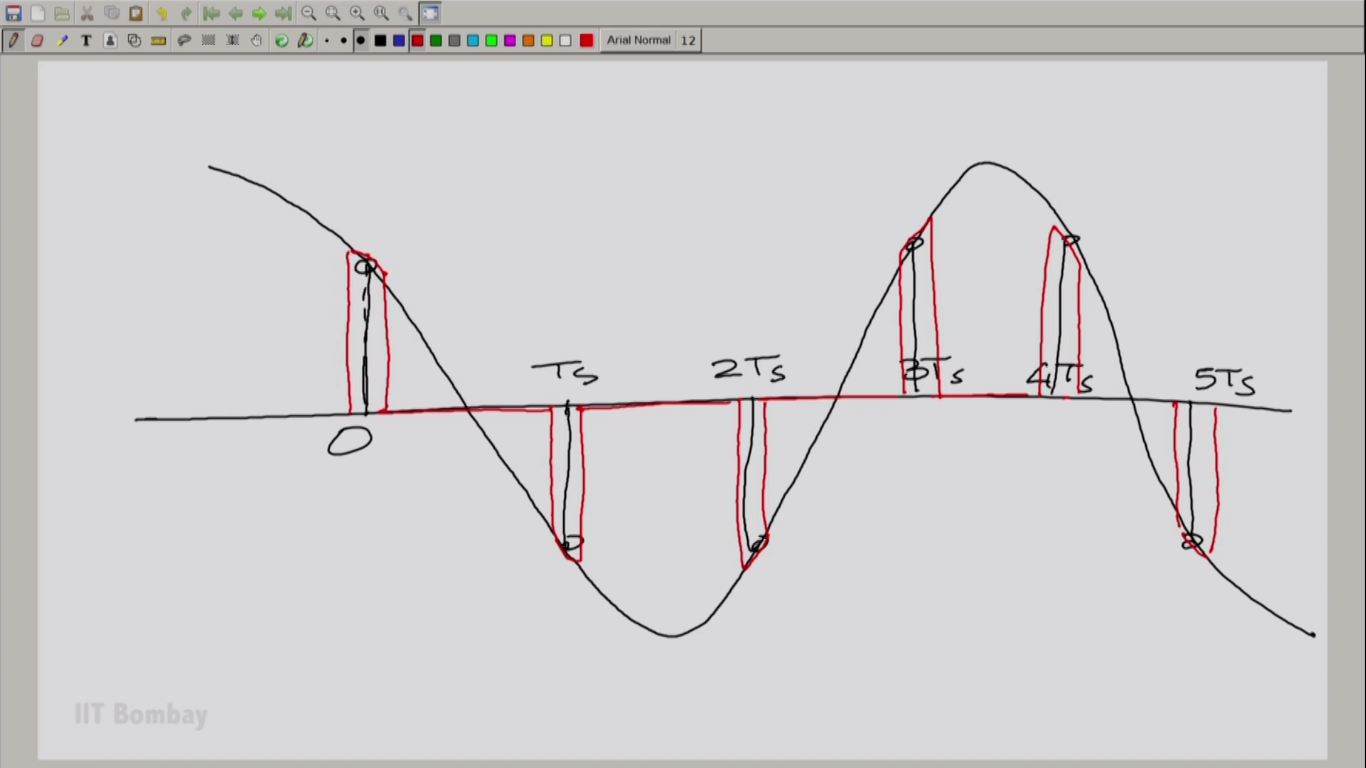
\includegraphics[scale=0.25]{curve.png}
\caption{The red curve represents the sampled signal while the black curve represents the original signal}
\end{figure}

\noindent The sampled curve can also be seen as the multiplication of the original signal (the sinusoid) with a train of very narrow pulses with unit height. However, note that these pulses are not impulses because they have a finite height (unit in this case).
\newline
Also note that this train of impulses is an even periodic function and hence, will have a Fourier series expansion of the form:-
\[
c_{0}+ \sum_{k=1}^{\infty} c_{k} \cos (\frac{2\pi}{T_{s}}kt + 0)
\]
The phase is $0$ because the function is even. $k=1$ represents the "fundamental" while $k$ \textgreater $1$ represents the "harmonics".
\newline
Using the previously learnt methods of computing the Fourier coefficients, 
\[
c_{0}=\frac{1\cdot \Delta}{T_{s}}
\]
and
\[
c_{k}=\frac{2}{T_{s}} \int \limits_{\frac{-\Delta}{2}}^{\frac{\Delta}{2}} 1 \cdot \cos (\frac{2\pi}{T_{s}}kt) dt
\]
\[
=\left.\frac{2}{T_{s}} \frac{\sin (\frac{2\pi}{T_{s}}kt)}{(\frac{2\pi}{T_{s}}k)} \right|_{\frac{-\Delta}{2}}^{\frac{\Delta}{2}}
\]
On substituting the limits and simplifying the value,
\[
c_{k}=\frac{2}{k} \sin (\frac{k\pi \Delta}{T_{s}})
\]
We see that the Fourier series becomes trivial for when $\Delta \rightarrow 0 $. To prevent this, we employ the same technique as we did in Module 1, we modify the pulse in such a way that the height is the inverse of the width. Note that this had converted our $pulse$ to an $impulse$.
\newline
The Fourier coefficients now become,
\[
c_{k}=\frac{1}{T_{s}}\cdot\frac{2}{\frac{k\Delta}{T_{s}}} \sin (\frac{k\pi \Delta}{T_{s}})
\]
Now, the Fourier expansion doesn't become trivial when $\Delta \rightarrow 0$. Rather, we can see that this is nothing but the sinc function.
\newline
Hence, we can see that 
\[
c_{k} \rightarrow \frac{2\pi}{T_{s}} \;\;\;\; as \;\;\;\; \Delta \rightarrow 0
\]

\subsection {Another Way of Sampling}
We can also write the complex Fourier expansion of the train of impulses. And proceed to multiply the original signal by the Fourier expansion (complex expansion) of the train of impulses. This is different from our previous method in the aspect that we have started with a train of impulses straightaway; instead of considering pulses and then converting them to impulses. This will give us the same result.
\newline
The complex Fourier expansion of this train of impulses is as follows; where $\gamma _{l}$ are the coefficients of each term of the expansion
\[
f(t)=\sum_{l=-\infty}^{\infty} \gamma_{l} \cdot exp(j \frac{2\pi}{T_{s}}lt)
\]
where f(t) is the train of impulses.
\newline
Let p(t) denote any one of the impulses which are periodically repeated over the entire $x$-axis to get f(t). Then for finding $\gamma_{l}$  :-
\[
\gamma_{l}= \frac{1}{T_{s}}\;\int \limits_{-\frac{T_{s}}{2}}^{\frac{T_{s}}{2}} \left( p(t)\cdot exp(-j \frac{2\pi}{T_{s}}lt) \right)  \; dt
\]
By the sifting property of the impulse, we can show that :-
\[
\gamma_{l}=\frac{1}{T_{s}}
\]
Hence, the complex Fourier expansion of the train of impulses is:-
\[
f(t)=\frac{1}{T_{s}}\;\sum_{l=-\infty}^{\infty} exp(j \frac{2\pi}{T_{s}}lt)
\]
which can further be simplified by taking the term for $l=0$ out of the sum and clubbing the terms with the same value of l, but with different signs together:-
\[
f(t)=\frac{1}{T_{s}}+\frac{1}{T_{s}}\;\sum_{l=1}^{\infty} exp(j \frac{2\pi}{T_{s}}lt) + exp(-j \frac{2\pi}{T_{s}}lt)
\]
This can be further simplified as:-
\[
f(t)=\frac{1}{T_{s}}+\frac{2}{T_{s}}\;\sum_{l=1}^{\infty} \cos (\frac{2\pi}{T_{s}}lt)
\]
This is the same as what we saw when we added all the impostor terms together!
\subsection{Conclusions}
We took two paths to analysing the imposter terms and the original sinusoid; the first was adding all these terms while the second was sampling the signal using impulses and analysing the resultant signal. For the analysis with impulses, we took two ways; the real Fourier series and the complex Fourier series expansions of the train of impulses.
\newline
Our observation is that both these processes are in fact, the same!
\newline
So, to conclude, bringing all these "impostor" sinusoids together with the original amounts to multiplying the original sinusoid with a uniform train of impulses located at the sampling instants!
\newline
Another indirect observation is that since the addition of all the impostor sinusoids with the original is the same as the sampling of the original sinusoid, they have constructive interference at the sampling instants (and hence return a finite value) and have a destructive interference everywhere else (hence the curve vanishes everywhere else).
\newline
These conclusions should be kept in mind as they are essential to the development of concepts that will be introduced further.

